\section{Probability of Satisfying Query}
\label{sec:prob_sat}

Now, we have an expression for delay that is built up using random variables for the values of $TF$ and $PL$.  The next useful formulation is providing an expression that describes the probability of a bottleneck flow satisfying its timeliness requirement considering the underlying distributions.  With this formulation, we can define scalability as a network in which the flow's probability of satisfiability exceeds some threshold $P_{thresh}$:
\begin{equation}
	P(D_i < T) \geq P_{thresh}
\label{eq:scal_definition}
\end{equation}

Once again, we have our total delay equation of a flow originating in node $i$:
\begin{equation}
	D_i = \frac{ k_{req} \cdot I_S \cdot CF \cdot TF_i}{W} + \frac{P_S \cdot DF \cdot (PL_i-1)}{W}
\end{equation}
Let us define two constants to simplify the expression:
\begin{eqnarray*}
	C_1 = \frac{k_{req} \cdot I_S \cdot CF}{W} \\
	C_2 = \frac{P_S \cdot DF}{W}
\end{eqnarray*}
Then, we can express the delay as
\begin{equation}
	D_i = C_1 \cdot TF_i + C_2 \cdot PL_i
\end{equation}
%As we showed in the last section, we can determine $i$ using the expected values for $TF_i$ and $PL_i$, so assuming that we adopt this value of $i$, we can drop the notation:
%\begin{equation}
%	D = C_1 \cdot TF + C_2 \cdot PL
%\end{equation}

The distribution of $D_i$ is determined by the convolution of $TF_i$ and $PL_i$:
\begin{equation}
	f_{D_i}(d) = \sum\limits_{pl=1}^{N-1} f_{PL_i}(pl) \cdot f_{TF_i}(\frac{d - C_2 \cdot pl}{C_1})
\label{eq:pdf_d_1}
\end{equation}
or
\begin{equation}
	f_{D_i}(d) = \sum\limits_{tf=1}^{N} f_{PL_i}(\frac{d - C_1 \cdot tf}{C_2}) \cdot f_{TF_i}(tf)
\label{eq:pdf_d_2}
\end{equation}

The cumulative distribution function of the delay, which is the ultimate goal to provide an expression for Equation (\ref{eq:scal_definition}), then, is
\begin{equation}
	F_{D_i}(d) = \sum\limits_{pl=1}^{N-1} f_{PL_i}(pl) \cdot F_{TF_i}(\frac{d - C_2 \cdot pl}{C_1})
	\label{eq:cdf_d_1}
\end{equation}

\begin{figure}
\begin{centering}
    \includegraphics[scale=0.4, clip=true, trim=15mm 65mm 20mm 65mm]{figures/PDF_D_125_line_net_B_1_KB.pdf}
    \caption{The PDF of delay for 1 KB flows originating in nodes 1 and 63 in a 125 node line network.}
    \label{fig:pdf_d_125_line_net_B_1_KB}
\end{centering}
\end{figure}

\begin{figure}
\begin{centering}
    \includegraphics[scale=0.4, clip=true, trim=15mm 65mm 20mm 65mm]{figures/CDF_D_125_line_net_B_1_KB.pdf}
    \caption{The CDF of delay for 1 KB flows originating in nodes 1 and 63 in a 125 node line network.}
    \label{fig:cdf_d_125_line_net_B_1_KB}
\end{centering}
\end{figure}

Using the definitions in Equations (\ref{eq:pdf_d_1}) and (\ref{eq:cdf_d_1}), we can visualize the distribution of delays of flows in the line network.  Figure \ref{fig:pdf_d_125_line_net_B_1_KB} shows the PDF of delays for flows of size $1 KB$ that originate in Node $1$ and in Node $63$ (the center node in the network), and Figure \ref{fig:cdf_d_125_line_net_B_1_KB} shows the CDF for the same network.  As we established in Section \ref{sec:bottleneck}, for this small data size, the bottleneck flow is likely to occur from the edge of the network.  This finding is validated by the distributions for $f_{D_1}$ and $F_{D_1}$ extending to higher delays than those of $f_{D_{63}}$ and $F_{D_{63}}$.

\begin{figure}
\begin{centering}
    \includegraphics[scale=0.4, clip=true, trim=15mm 65mm 20mm 65mm]{figures/PDF_D_125_line_net_B_18_KB.pdf}
    \caption{The PDF of delay for 18 KB flows originating in nodes 1 and 63 in a 125 node line network.}
    \label{fig:pdf_d_125_line_net_B_18_KB}
\end{centering}
\end{figure}

\begin{figure}
\begin{centering}
    \includegraphics[scale=0.4, clip=true, trim=15mm 65mm 20mm 65mm]{figures/CDF_D_125_line_net_B_18_KB.pdf}
    \caption{The CDF of delay for 18 KB flows originating in nodes 1 and 63 in a 125 node line network.}
    \label{fig:cdf_d_125_line_net_B_18_KB}
\end{centering}
\end{figure}

Figures \ref{fig:pdf_d_125_line_net_B_18_KB} and \ref{fig:cdf_d_125_line_net_B_18_KB} provide the distributions of flows originating from nodes on the edge and center of the network as well, except for an expected data requirement of $18 KB$.  Here, we see the ordering of the delay distributions is reversed, also as expected from the findings in Section \ref{sec:bottleneck}.

%\subsection{Expanded expression for $i=1$}
%For $i=1$, the distribution is approximately (we drop the first term):
%\begin{eqnarray*}
%	f_{D}^1(d) &=& \sum\limits_{pl=1}^{N-1} \{ (\frac{pl-1}{N} ) \cdot \\
%		& & [ \sum\limits_{k=1}^{\frac{N}{2}-1} \frac{\frac{1}{2}-\frac{1}{N}}{\frac{N}{2} - 1} \cdot \frac{1}{\sigma(k)}\phi(\frac{x^* - \mu(k)}{\sigma(k)}) \\
%		&+& \frac{1}{2} \cdot \frac{1}{\sigma(k)} \phi ( \frac{x^* - \mu(\frac{N}{2})}{\sigma(\frac{N}{2})}) ] \}
%\end{eqnarray*}
%where $x^*$ is $(d - C_2 \cdot pl)/C_1$
%
%For $i=1$, the distribution is approximately:
%\begin{eqnarray*}
%	F_{D}^1(d) &=& \sum\limits_{pl=1}^{N-1} \{ (\frac{pl-1}{N} ) \cdot \\
%		& & [ \sum\limits_{k=1}^{\frac{N}{2}-1} \frac{\frac{1}{2}-\frac{1}{N}}{\frac{N}{2} - 1} \cdot \frac{1}{\sigma(k)}\Phi(\frac{x^* - \mu(k)}{\sigma(k)}) \\
%		&+& \frac{1}{2} \cdot \frac{1}{\sigma(k)} \Phi ( \frac{x^* - \mu(\frac{N}{2})}{\sigma(\frac{N}{2})}) ] \}
%\end{eqnarray*}
%where $x^*$ is $(d - C_2 \cdot pl)/C_1$

%\begin{figure}
%\begin{centering}
%    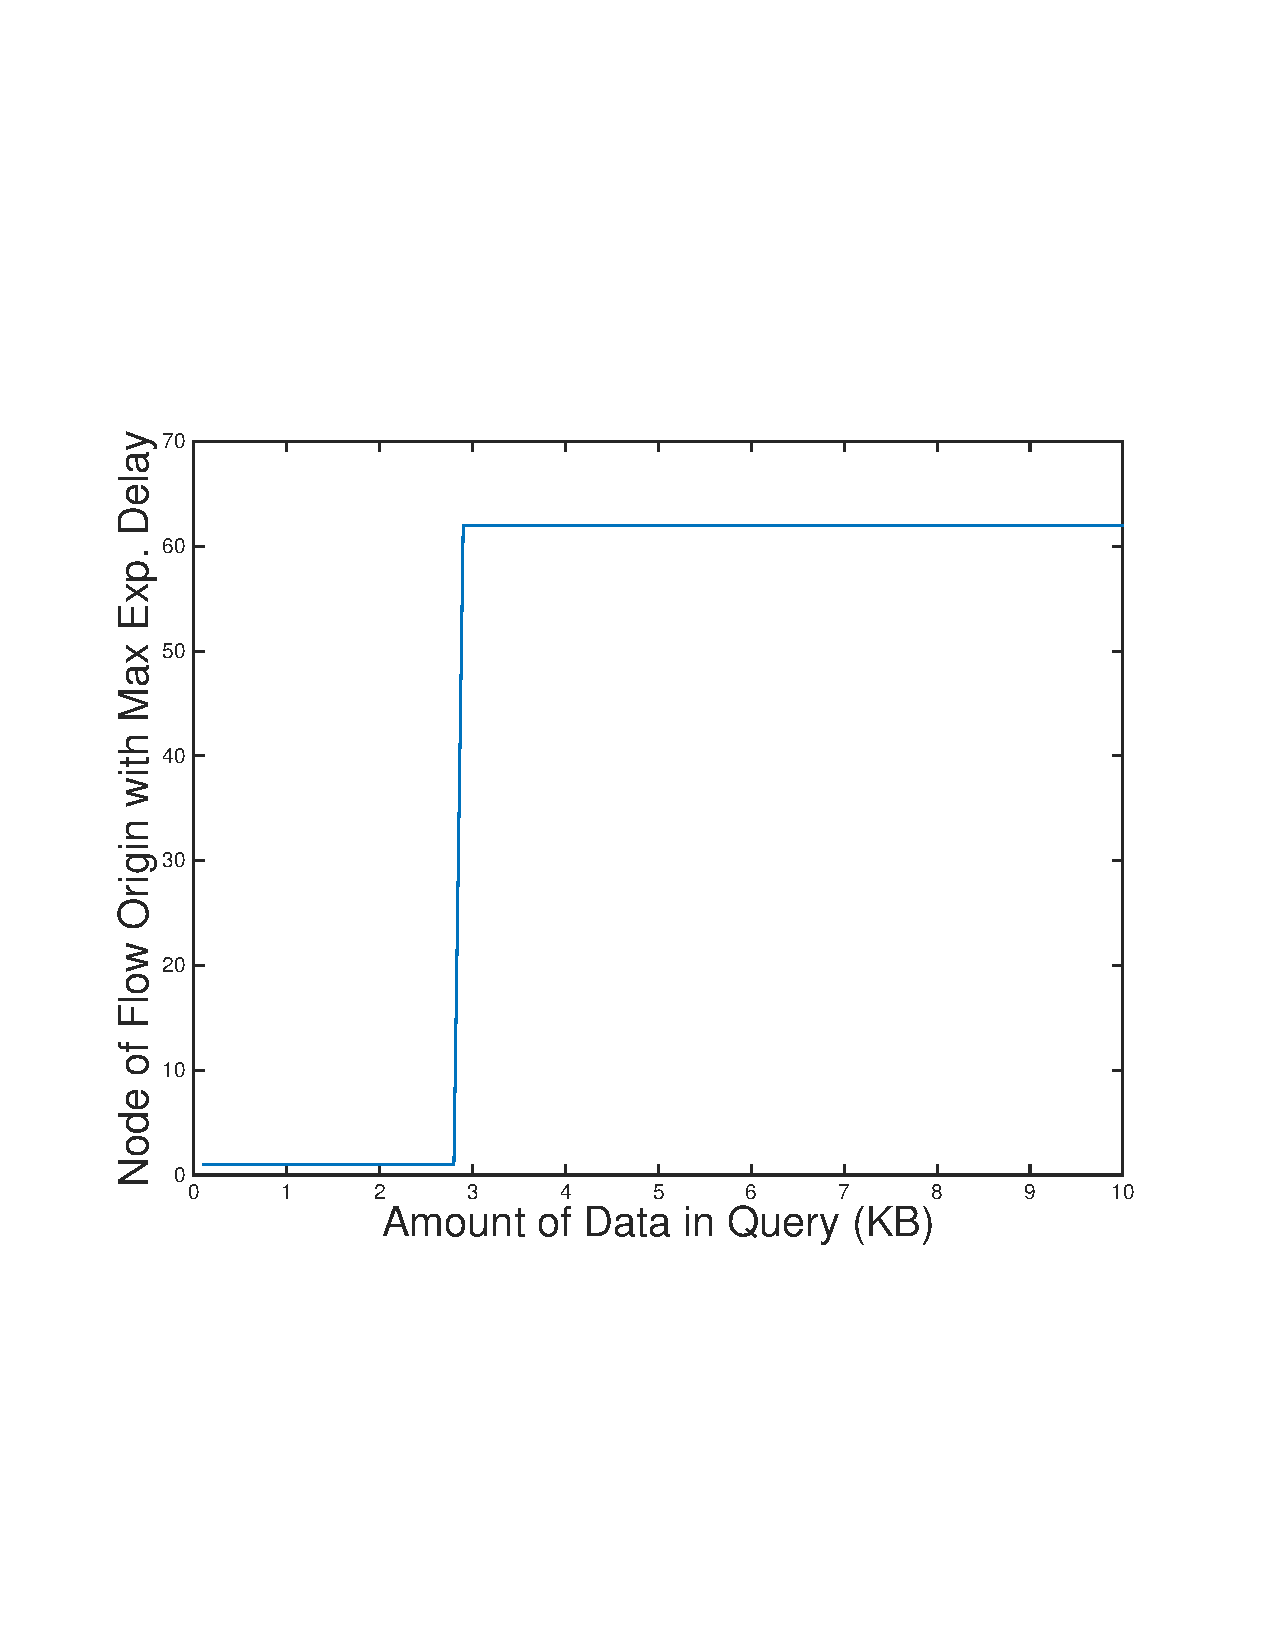
\includegraphics[scale=0.4, clip=true, trim=15mm 65mm 20mm 65mm]{figures/max_i_line_net_125.pdf}
%    \caption{The value of $i$ (origin of a flow) that causes the maximum expected delay.}
%    \label{fig:max_i_line_net}
%\end{centering}
%\end{figure}


